% !TeX program = pdflatex
\documentclass[12pt,a4paper]{article}

% Essential packages
\usepackage[utf8]{inputenc}
\usepackage[T1]{fontenc}
\usepackage[polish]{babel}
\usepackage{csquotes}
\usepackage{amsmath}
\usepackage{hyperref}
\usepackage{xcolor}
\usepackage{geometry}
\usepackage{booktabs}
\usepackage{float}  
\usepackage{array}    
\usepackage[backend=biber,style=numeric,sorting=none]{biblatex}
\usepackage{graphicx}
\usepackage{tocloft}  % For customizing table of contents
\usepackage{enumitem} % For better list formatting
\usepackage{listings} % For code listings with line wrapping

\geometry{
    a4paper,
    margin=2.5cm
}

% Listings package configuration
\lstset{
  basicstyle=\ttfamily\small,
  breakatwhitespace=false,
  breaklines=true,
  postbreak=\mbox{\textcolor{red}{$\hookrightarrow$}\space},
  showstringspaces=false
}


% Table of contents settings
\renewcommand{\cftsecleader}{\cftdotfill{\cftdotsep}}
\renewcommand{\cftsubsecleader}{\cftdotfill{\cftdotsep}}
\setcounter{tocdepth}{2}  % Show sections and subsections in TOC
\setcounter{secnumdepth}{2}  % Number sections and subsections

% Hyperref settings
\hypersetup{
    colorlinks=true,
    linkcolor=blue,
    filecolor=magenta,
    urlcolor=cyan,
    pdftitle={Raport końcowy: Równoległy System Analizy Roślinności Sentinel-2},
    pdfauthor={Adrian Rybaczuk, Bartosz Cylwik},
    pdfsubject={Przetwarzanie Rozproszone i Równoległe},
    pdfkeywords={Sentinel-2, NDVI, NDMI, Przetwarzanie Równoległe, Python, GUI}
}


\title{Projekt zaliczeniowy\\\large Raport końcowy}
\author{Zespół Projektowy nr 1 \\
    \begin{tabular}{ll}
        \textbf{Adrian Rybaczuk} & \textbf{318483} \\
        \textbf{Bartek Cylwik} & \textbf{325457} \\
    \end{tabular}
}
\date{\today}


% Bibliography file
\addbibresource{references.bib}
\selectlanguage{polish} % Set language to Polish
\begin{document}

\maketitle

\begin{abstract}
  Niniejszy raport przedstawia podsumowanie projektu grupowego, systemu do równoległego przetwarzania obrazów satelitarnych Sentinel-2, umożliwiającego efektywną analizę zmian roślinności z wykorzystaniem wskaźników NDVI i NDMI oraz przyjaznego interfejsu graficznego. Projekt skupia się na implementacji i porównaniu różnych strategii przetwarzania równoległego, w tym obliczeń na GPU oraz wielowątkowych obliczeń na CPU, w celu zbadania ich wydajności i praktycznej użyteczności w zależności od charakterystyki problemu.
  \end{abstract}
  

\tableofcontents
\newpage


\section{Wprowadzenie}
Celem projektu była implementacja (wraz z GUI) systemu równoległego / rozproszonego mechanizmu wyliczania indeksów wilgotności (NDMI) i wegetacji (NDVI) roślin na zobrazowaniach satelitarnych Sentinel-2 do stwierdzenia występowania lub zaniku roślinności na wskazanym obszarze.
Na podstawie tak zdefiniowanego zadania mogliśmy wyznaczyć poszczególne elementy projektu do realizacji:
\begin{itemize}
    \item Uzyskanie wskaźników NDVI i NDMI
    \begin{itemize}
        \item Research na temat wskaźników NDVI i NDMI
        \item Pobranie niezbędnych wskaźników z zobrazowania satelitarnego Sentinel-2
        \item Zapisanie danych pobranych z API jako "cache" w celu uniknięcia ponownego pobierania danych
        \item Identyfikacja potęcjalnych problemów związanych z przetwarzaniem danych
        \item Przeprowadzenie obliczeń wskaźników
    \end{itemize}
    \item Interfejs graficzny
    \begin{itemize}
        \item Ekran uwierzytelniania z API Sentinel-Hub
        \item Ekran pozwalający na wybór zakresu czasowego oraz obszaru analizy
        \item Ekran z wynikami analizy w postaci mapy z zaznaczonymi obszarami roślinności
    \end{itemize}
    \item Równoległe przetwarzanie
    \begin{itemize}
        \item Wybranie obszarów programu wymagających przetworzenia równoległego / rozproszonego
        \item Wybranie pomiedzy przetwarzaniem na CPU a GPU
        \item Implementacja mechanizmu równoległego / rozproszonego przetwarzania
    \end{itemize}
    \item Wybranie technologi do realizacji projektu
\end{itemize}

\newpage

\section{Kroki podjęte na początku pracy}

\subsection{Research wskaźników NDVI i NDMI}

Aby uzyskać wskaźniki NDVI i NDMI, rozpoczęliśmy od analizy literatury i dokumentacji dotyczącej tych indeksów, przechodząc od ogólnych informacji do szczegółowych aspektów ich wyznaczania.

\textbf{NDVI} (Normalized Difference Vegetation Index) \cite{ndvi_docs} jest prostym wskaźnikiem ilościowym służącym do klasyfikacji wegetacji roślin. Jego wartość mieści się w przedziale od $-1$ do $1$:
\begin{itemize}
    \item Wartości ujemne (zbliżone do $0$) wskazują na obecność wody.
    \item Zakres $-0.1$ do $0.1$ odpowiada obszarom jałowym (skały, piasek, śnieg).
    \item Przedział $0.2$ do $0.4$ oznacza niską roślinność (zarośla, łąki).
    \item Wysokie wartości (bliskie $1$) wskazują na bujną roślinność (np. lasy deszczowe).
\end{itemize}

Dzięki temu NDVI jest dobrym wskaźnikiem obecności i kondycji roślinności na danym obszarze.

Wskaźnik NDVI definiuje się wzorem:
\[
\mathrm{NDVI} = \mathrm{Index}(\mathrm{NIR}, \mathrm{RED}) = \frac{\mathrm{NIR} - \mathrm{RED}}{\mathrm{NIR} + \mathrm{RED}}
\]

W przypadku danych Sentinel-2, indeks ten wyznaczamy na podstawie kanałów B8 (NIR) i B4 (RED):
\[
\mathrm{NDVI} = \mathrm{Index}(\mathrm{B8}, \mathrm{B4}) = \frac{\mathrm{B8} - \mathrm{B4}}{\mathrm{B8} + \mathrm{B4}}
\]

\textbf{NDMI} (Normalized Difference Moisture Index) \cite{ndmi_docs} jest znormalizowanym wskaźnikiem wilgotności który do wyznaczenia wilgotności wykorzystuje pasma NIR i SWIR.
\begin{itemize}
    \item Wartosci ujemne (zblizone do -1) wskazuja na bardzo suche obszary (brak roslnosci, pustynia, obszary zabudowane)
    \item Wartosci od -0.2 do 0.2 wskazuja na glebe wysychającą (rzadka trawa, trawy wysychające, krzewy w stanie stresu wodnego)
    \item Wartosci ponizej do 0.2 do 0.4 odpowiadaja umiarkowanemu nawodnieniu (trawy, pastwiska)
    \item Wartosci od 0.4  Wskazują na obszary o zdrowy stan nawodnienia (uprawy w pełni sezonu wegetacyjnego, lasy liściaste w strefie umiarkowanej) 
    \item Wartosci powyzej 0.4 wskazuja na obszary o wysokiej wilgotnosci (lasy deszczowe, obszary podmokłe)
\end{itemize}

Wskaźnik NDMI definiujemy wzorem:
\[
\mathrm{NDMI} = \mathrm{Index}(\mathrm{NIR}, \mathrm{SWIR}) = \frac{\mathrm{NIR} - \mathrm{SWIR}}{\mathrm{NIR} + \mathrm{SWIR}}
\]

W przypadku danych Sentinel-2, indeks ten wyznaczamy na podstawie kanałów B8 (NIR) i B11 (SWIR):
\[
\mathrm{NDMI} = \mathrm{Index}(\mathrm{B8}, \mathrm{B11}) = \frac{\mathrm{B8} - \mathrm{B11}}{\mathrm{B8} + \mathrm{B11}}
\]

\subsection{RED, NIR, SWIR czyli B4, B8, B11}

\textbf{RED} to czerwony kanał światła, silnie odbijany przez martwe liście. Wykorzystuje się go do identyfikacji typów roślinności, gleb oraz obszarów zabudowanych. Charakteryzuje się ograniczoną penetracją w wodzie i słabym odbiciem od liści zawierających chlorofil (żywe liście).

W satelitach Sentinel-2 kanał RED odpowiada pasmu B4: \cite{sentinel2_band_B4}
\begin{itemize}
    \item Rozdzielczość: 10 m/px
    \item Centralna długość fali: 665 nm
    \item Szerokość pasma: 30 nm
\end{itemize}

\textbf{NIR} (Near Infrared) to bliska podczerwień, która dobrze obrazuje linie brzegowe oraz zawartość biomasy.

W Sentinel-2 kanał NIR odpowiada pasmu B8: \cite{sentinel2_band_B8}
\begin{itemize}
    \item Rozdzielczość: 10 m/px
    \item Centralna długość fali: 842 nm
    \item Szerokość pasma: 115 nm
\end{itemize}

\textbf{SWIR} (Short-Wave Infrared) jest to fala wysokowrażliwa na zawartość wody w obiektach. Dlatego jest dobrym wskaźnikiem wilgotności.

W Sentinel-2 kanał SWIR odpowiada pasmu B11: \cite{sentinel2_band_B11}
\begin{itemize}
    \item Rozdzielczość: 20 m/px
    \item Centralna długość fali: 1610 nm
    \item Szerokość pasma: 130 nm
\end{itemize}

\subsection{Problem Różnych Rozdzielczości}
Istotną informacją na temat pasm dostarczanych przez Sentinel-2 jest ich natywna rozdzielczość. Możemy zauważyć różnice w rozdzielczości między kanałami, np. B4 i B8 (10m) a B11 (20m). Naszą początkową hipotezą była konieczność ręcznego przeskalowania danych (downscalingu) w celu ich ujednolicenia.

Jednakże, w toku prac odkryliśmy, że API Sentinel Hub, z którego korzystamy, dostarcza wszystkie zamówione pasma już przeskalowane do wspólnej, najwyższej rozdzielczości (w naszym przypadku 10m). Mechanizm ten, znany jako co-rejestracja, jest standardową praktyką w przetwarzaniu danych satelitarnych i znacznie uprościł nasz proces przetwarzania wstępnego. Pozwoliło nam to operować na danych o najwyższej możliwej szczegółowości bez ryzyka utraty informacji, która mogłaby wystąpić przy ręcznym zmniejszaniu rozdzielczości.

\subsection{Zrównoleglenie / rozproszenie obliczeń}
W związku z tym, że chcieliśmy, by aplikacja działała na jednym komputerze, wybraliśmy ścieżkę zrównoleglenia obliczeń. Zadanie obliczania wskaźników polega na wykonaniu prostych operacji arytmetycznych dla milionów pikseli. Operacje te są powtarzalne i niezależne od siebie, co czyni je idealnym kandydatem do zrównoleglenia.

Naszą początkową hipotezą było, że obliczenia na GPU, ze względu na ich masowo równoległą architekturę, będą najwydajniejszym rozwiązaniem. Jednakże, aby przeprowadzić rzetelną analizę i zrozumieć kompromisy związane z różnymi podejściami, postanowiliśmy zaimplementować i porównać trzy odrębne strategie obliczeniowe:
\begin{enumerate}
    \item \textbf{Przetwarzanie na GPU} z wykorzystaniem języka Taichi, aby zbadać potencjał masowego zrównoleglenia.
    \item \textbf{Równoległe przetwarzanie na CPU} z wykorzystaniem modułu \texttt{multiprocessing} i pamięci dzielonej, aby ocenić skalowalność na wielordzeniowych procesorach.
    \item \textbf{Jednowątkowe przetwarzanie na CPU} z wykorzystaniem wysoce zoptymalizowanej biblioteki NumPy, służące jako kluczowy punkt odniesienia (baseline) do oceny narzutu (overhead) metod równoległych.
\end{enumerate}
Taki zakres implementacji pozwolił na dogłębną analizę wydajności i zidentyfikowanie, która metoda jest optymalna w zależności od charakterystyki problemu, co stanowi główny trzon niniejszego raportu.

\subsection{Następnym krokiem będzie uzyskanie dostępu do danych z Sentinel-2}

Do tego celu skorzystaliśmy z API Sentinel-Hub. \cite{sentinel2_api_docs} 
Udostępnia on dane z satelity poprzez API dopiero po uwierzytelnieniu. 
W tym celu musielismy przejść przez process opisany tutaj \cite{sentinel2_api_docs_auth}.
Po jego przejsciu mamy dostep do Client ID oraz Client Secret które wykorzystamy do połączenia się z API.

API posiada reate limiting które są w miare restrykcyjne. \cite{sentinel2_api_auth_rate_limiting}
Z tego też powodu zamierzamy wykorzystać cache do przechowywania pobranych już danych.
Z natury projektu i dania sobie możliwości testowania wyników zamierzamy przechowywać nieprzetworzone dane zamiast obliczonych już wyników.
Pomoże nam to przeprowadzić testy i wprowadzić poprawki w przyszłości.

\subsection{Wybór technologii}

Jako że określiliśmy już dokładniej ramy projektu możemy potwierdzić wybrane przez nas technologie. 
Ogólny język implementacji to Python.
Do pobierania danych z api wykorzystaliśmy bibliotekę SentinelHub. Która udosptępnia już gotowe funkcje pozwalające zautoryzować się z api oraz pobrać dane.
Do gui wykorzystaliśmy Tkinter podstawową i dosyć prostą bibliotekę do tworzenia interfejsu graficznego.
Do prezentacji mapy wykorzystaliśmy TkinterMapView.
Do zrównoleglenia obliczeń skorzystamy z Taichi Lang \cite{taichi_lang_docs} którego zaembedujemy w pythonie.
Jest to język programowania osadzony w pythonnie stworzony do wysokowydajnych obliczeń.
Jego zaletą jest to że kod napisany raz przekąpiluje się na wiele różnych platform.

\newpage

\section{Przebieg procesu w aplikacji}
Aplikacja została zaprojektowana z myślą o prostocie i intuicyjności obsługi. Interakcja użytkownika z systemem przebiega w kilku logicznych krokach:
\begin{enumerate}
    \item \textbf{Uwierzytelnianie:} Po uruchomieniu aplikacji, użytkownik jest proszony o podanie danych uwierzytelniających do API Sentinel Hub. Aplikacja bezpiecznie przechowuje te dane w zaszyfrowanym pliku, aby przy kolejnych uruchomieniach wymagać jedynie podania hasła.
    \item \textbf{Główny widok mapy:} Po pomyślnym zalogowaniu, użytkownik przechodzi do głównego interfejsu, który składa się z dwóch głównych paneli: interaktywnej mapy satelitarnej oraz panelu na wyniki.
    \item \textbf{Wybór obszaru i parametrów:} Użytkownik może swobodnie nawigować po mapie (przesuwać, przybliżać), aby wybrać interesujący go obszar. W górnym panelu dostępne są kontrolki do wyboru zakresu dat oraz metody przetwarzania (GPU lub CPU).
    \item \textbf{Pobieranie danych:} Po kliknięciu przycisku "Fetch Data", aplikacja wysyła zapytanie do API Sentinel Hub o pasma B4, B8, B11 oraz maskę danych dla widocznego na ekranie obszaru. Pobrane dane są zapisywane w lokalnym folderze \texttt{data}, który pełni rolę pamięci podręcznej (cache), aby uniknąć ponownego pobierania tych samych danych.
    \item \textbf{Obliczenia i wizualizacja:} Po pobraniu danych, aktywują się przyciski "Calculate NDVI" i "Calculate NDMI". Kliknięcie jednego z nich uruchamia obliczenia w osobnym wątku (aby nie blokować interfejsu), wykorzystując wybraną przez użytkownika metodę (GPU lub CPU). Po zakończeniu obliczeń, w prawym panelu wyświetlana jest mapa cieplna (heatmap) wskaźnika wraz z legendą.
    \item \textbf{Moduł testowy:} Z widoku mapy użytkownik może przejść do dedykowanego panelu testowego, który pozwala na uruchomienie serii testów wydajnościowych i wygenerowanie szczegółowych wykresów porównujących zaimplementowane metody obliczeniowe.
\end{enumerate}

\section{Równoległe przetwarzanie}

\subsection{Które obliczenia i dlaczego postanowiliśmy zrównoleglić}
Głównym kandydatem do zrównoleglenia w naszym projekcie były obliczenia wskaźników NDVI i NDMI. Decyzja ta wynikała z charakterystyki problemu:
\begin{itemize}
    \item \textbf{Niezależność danych (Data Parallelism):} Wartość wskaźnika dla każdego piksela obrazu satelitarnego jest obliczana wyłącznie na podstawie wartości pasm dla tego samego piksela. Nie ma żadnych zależności między sąsiednimi pikselami.
    \item \textbf{Duża skala problemu:} Obrazy satelitarne mogą składać się z milionów, a nawet dziesiątek milionów pikseli. Wykonywanie operacji na tak dużej liczbie danych w sposób sekwencyjny może być czasochłonne.
    \item \textbf{Powtarzalność operacji:} Ten sam, prosty wzór matematyczny \((a-b)/(a+b)\) jest stosowany dla każdego piksela.
\end{itemize}
Te cechy sprawiają, że problem ten jest klasyfikowany jako "wstydliwie równoległy" (embarrassingly parallel), co czyni go idealnym do zastosowania technik przetwarzania równoległego w celu skrócenia czasu obliczeń.

\subsection{Jak dokonaliśmy zrównoleglenia obliczeń}
Aby przeprowadzić kompleksową analizę, zaimplementowaliśmy trzy różne strategie obliczeniowe:

\subsubsection{Przetwarzanie na GPU z użyciem Taichi Lang}
Taichi to język programowania osadzony w Pythonie, działający jako kompilator JIT (Just-In-Time). Pozwala on na pisanie funkcji w składni zbliżonej do Pythona, które są następnie kompilowane do wysoce zoptymalizowanego kodu maszynowego dla różnych architektur, w tym GPU (poprzez backendy takie jak CUDA, DirectX, Metal). W naszej implementacji, kernel Taichi wykonuje operację \((a-b)/(a+b)\) dla całej tablicy danych, wykorzystując tysiące rdzeni GPU do jednoczesnego przetworzenia wielu pikseli.

\subsubsection{Równoległe przetwarzanie na CPU z użyciem `multiprocessing`}
Aby wykorzystać wielordzeniową architekturę nowoczesnych procesorów, użyliśmy wbudowanego w Pythona modułu \texttt{multiprocessing}. Kluczowym wyzwaniem w tym podejściu jest narzut związany z komunikacją między procesami i kopiowaniem danych. Aby go zminimalizować, zaimplementowaliśmy mechanizm oparty na \textbf{pamięci dzielonej (Shared Memory)}. Zamiast wysyłać kopie fragmentów obrazu do każdego procesu roboczego, tworzymy w pamięci RAM jeden, duży segment, do którego wszystkie procesy mają bezpośredni dostęp. Każdy proces otrzymuje jedynie informację o fragmencie (zakresie wierszy), który ma przetworzyć, co drastycznie redukuje koszt komunikacji.

\subsubsection{Jednowątkowe przetwarzanie na CPU z użyciem NumPy}
Jako punkt odniesienia, stworzyliśmy również implementację jednowątkową. Nie jest to jednak prosta pętla w Pythonie. Wykorzystaliśmy bibliotekę NumPy, której operacje na tablicach (np. dodawanie, odejmowanie) nie są wykonywane przez interpreter Pythona, ale przez wysoce zoptymalizowane, prekompilowane procedury w językach C i Fortran. Dzięki temu, operacje te są wykonywane bardzo szybko na jednym rdzeniu CPU i stanowią silny baseline do porównań z metodami równoległymi.

\newpage

\section{Platforma Testowa}
Wszystkie testy wydajnościowe zostały przeprowadzone na jednolitej platformie sprzętowej, aby zapewnić spójność i porównywalność wyników. Poniższa specyfikacja dokumentuje konfigurację komputera użytego do testów. Zrozumienie kontekstu sprzętowego jest kluczowe dla poprawnej interpretacji wyników, ponieważ wydajność zależy od wielu czynników, takich jak moc obliczeniowa CPU i GPU, szybkość pamięci RAM czy przepustowość magistrali PCIe.

\begin{description}
    \item[System Operacyjny:] Windows 10 (AMD64)
    \item[Procesor (CPU):] AMD Ryzen 9 3900X
    \item[Szczegóły CPU:] 12 rdzeni fizycznych / 24 wątki, Taktowanie bazowe: 3.8 GHz, Cache L2: 6 MB, Cache L3: 64 MB
    \item[Pamięć RAM:] 64 GB DDR4
    \item[Karta Graficzna (GPU):] NVIDIA GeForce RTX 2070 SUPER
\end{description}

\textit{Uwaga: Na wydajność, zwłaszcza w przypadku obliczeń na GPU, mają również wpływ czynniki nieujęte w powyższej specyfikacji, takie jak wersja i przepustowość magistrali PCIe, szybkość pamięci VRAM oraz ogólne obciążenie systemu podczas testów.}

\section{Jakie wyniki uzyskaliśmy}
W celu oceny wydajności zaimplementowanych metod, przeprowadziliśmy serię testów na dedykowanej platformie testowej. Testy polegały na mierzeniu czasu wykonania obliczeń dla danych o różnej rozdzielczości oraz analizie zużycia pamięci. Poniższe wykresy prezentują zebrane wyniki.

\begin{figure}[H]
    \centering
    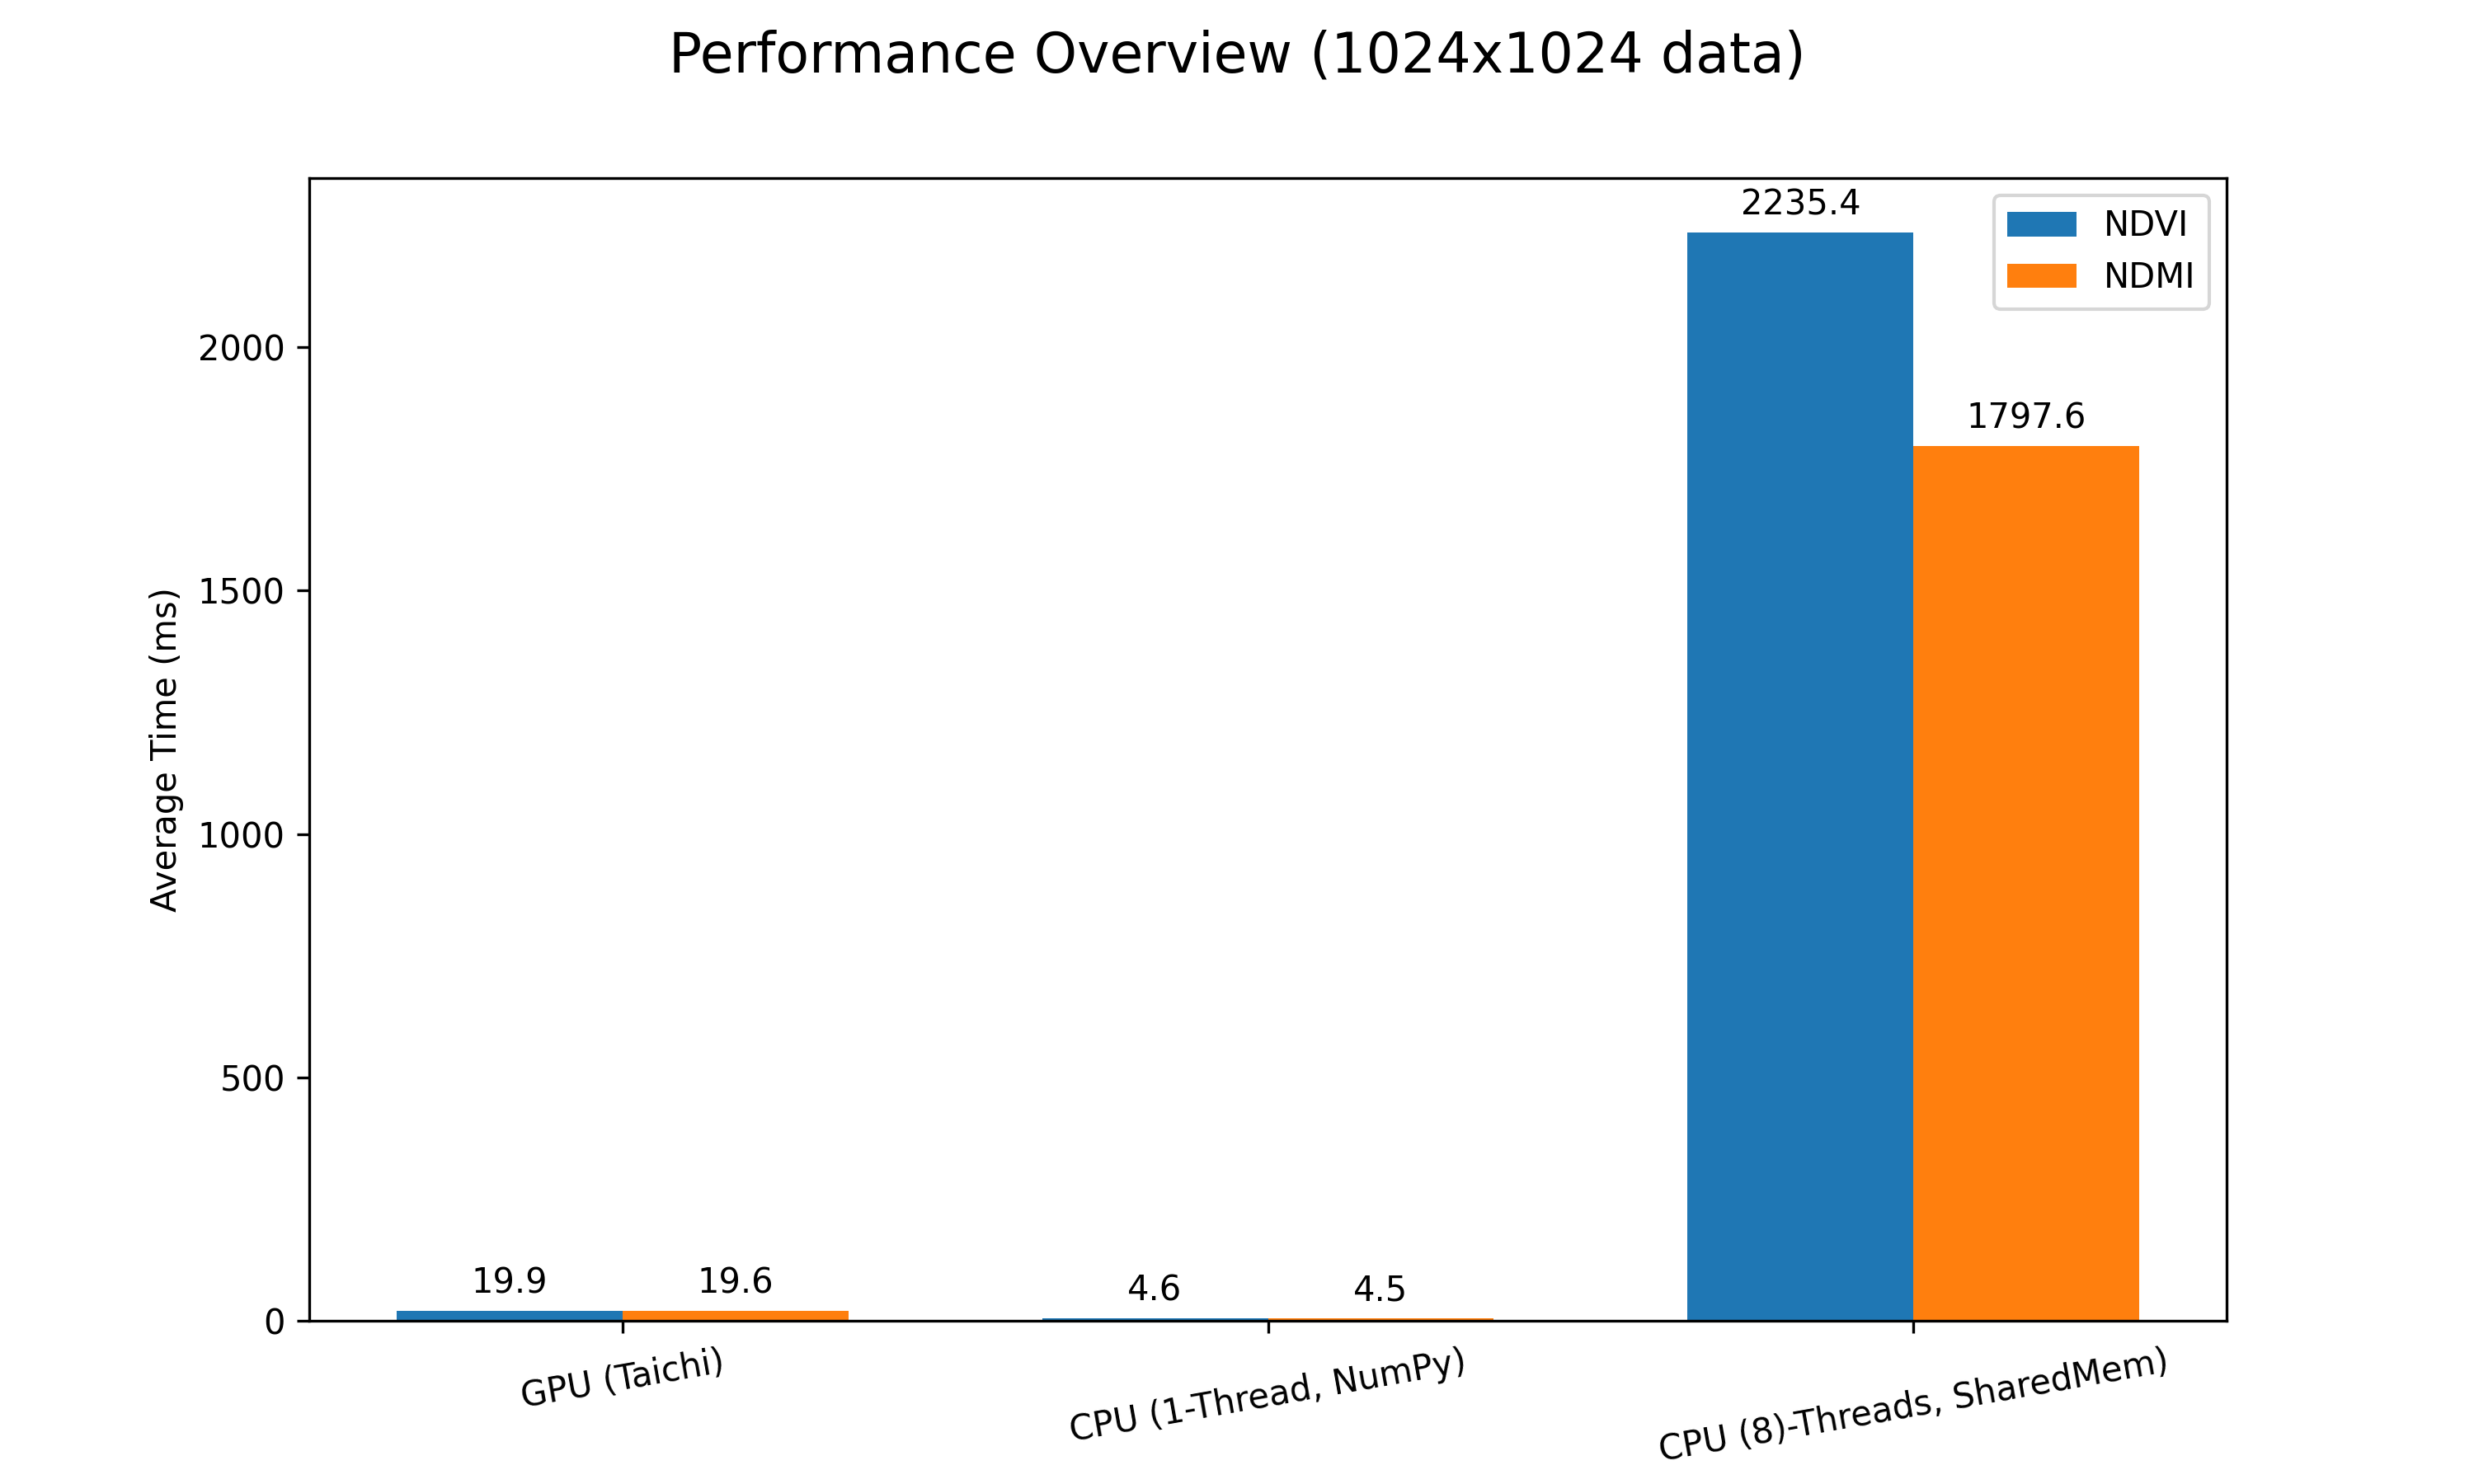
\includegraphics[width=0.8\textwidth]{charts/01_performance_overview.png}
    \caption{Przegląd wydajności dla danych 1024x1024.}
    \label{fig:overview}
\end{figure}

\begin{figure}[H]
    \centering
    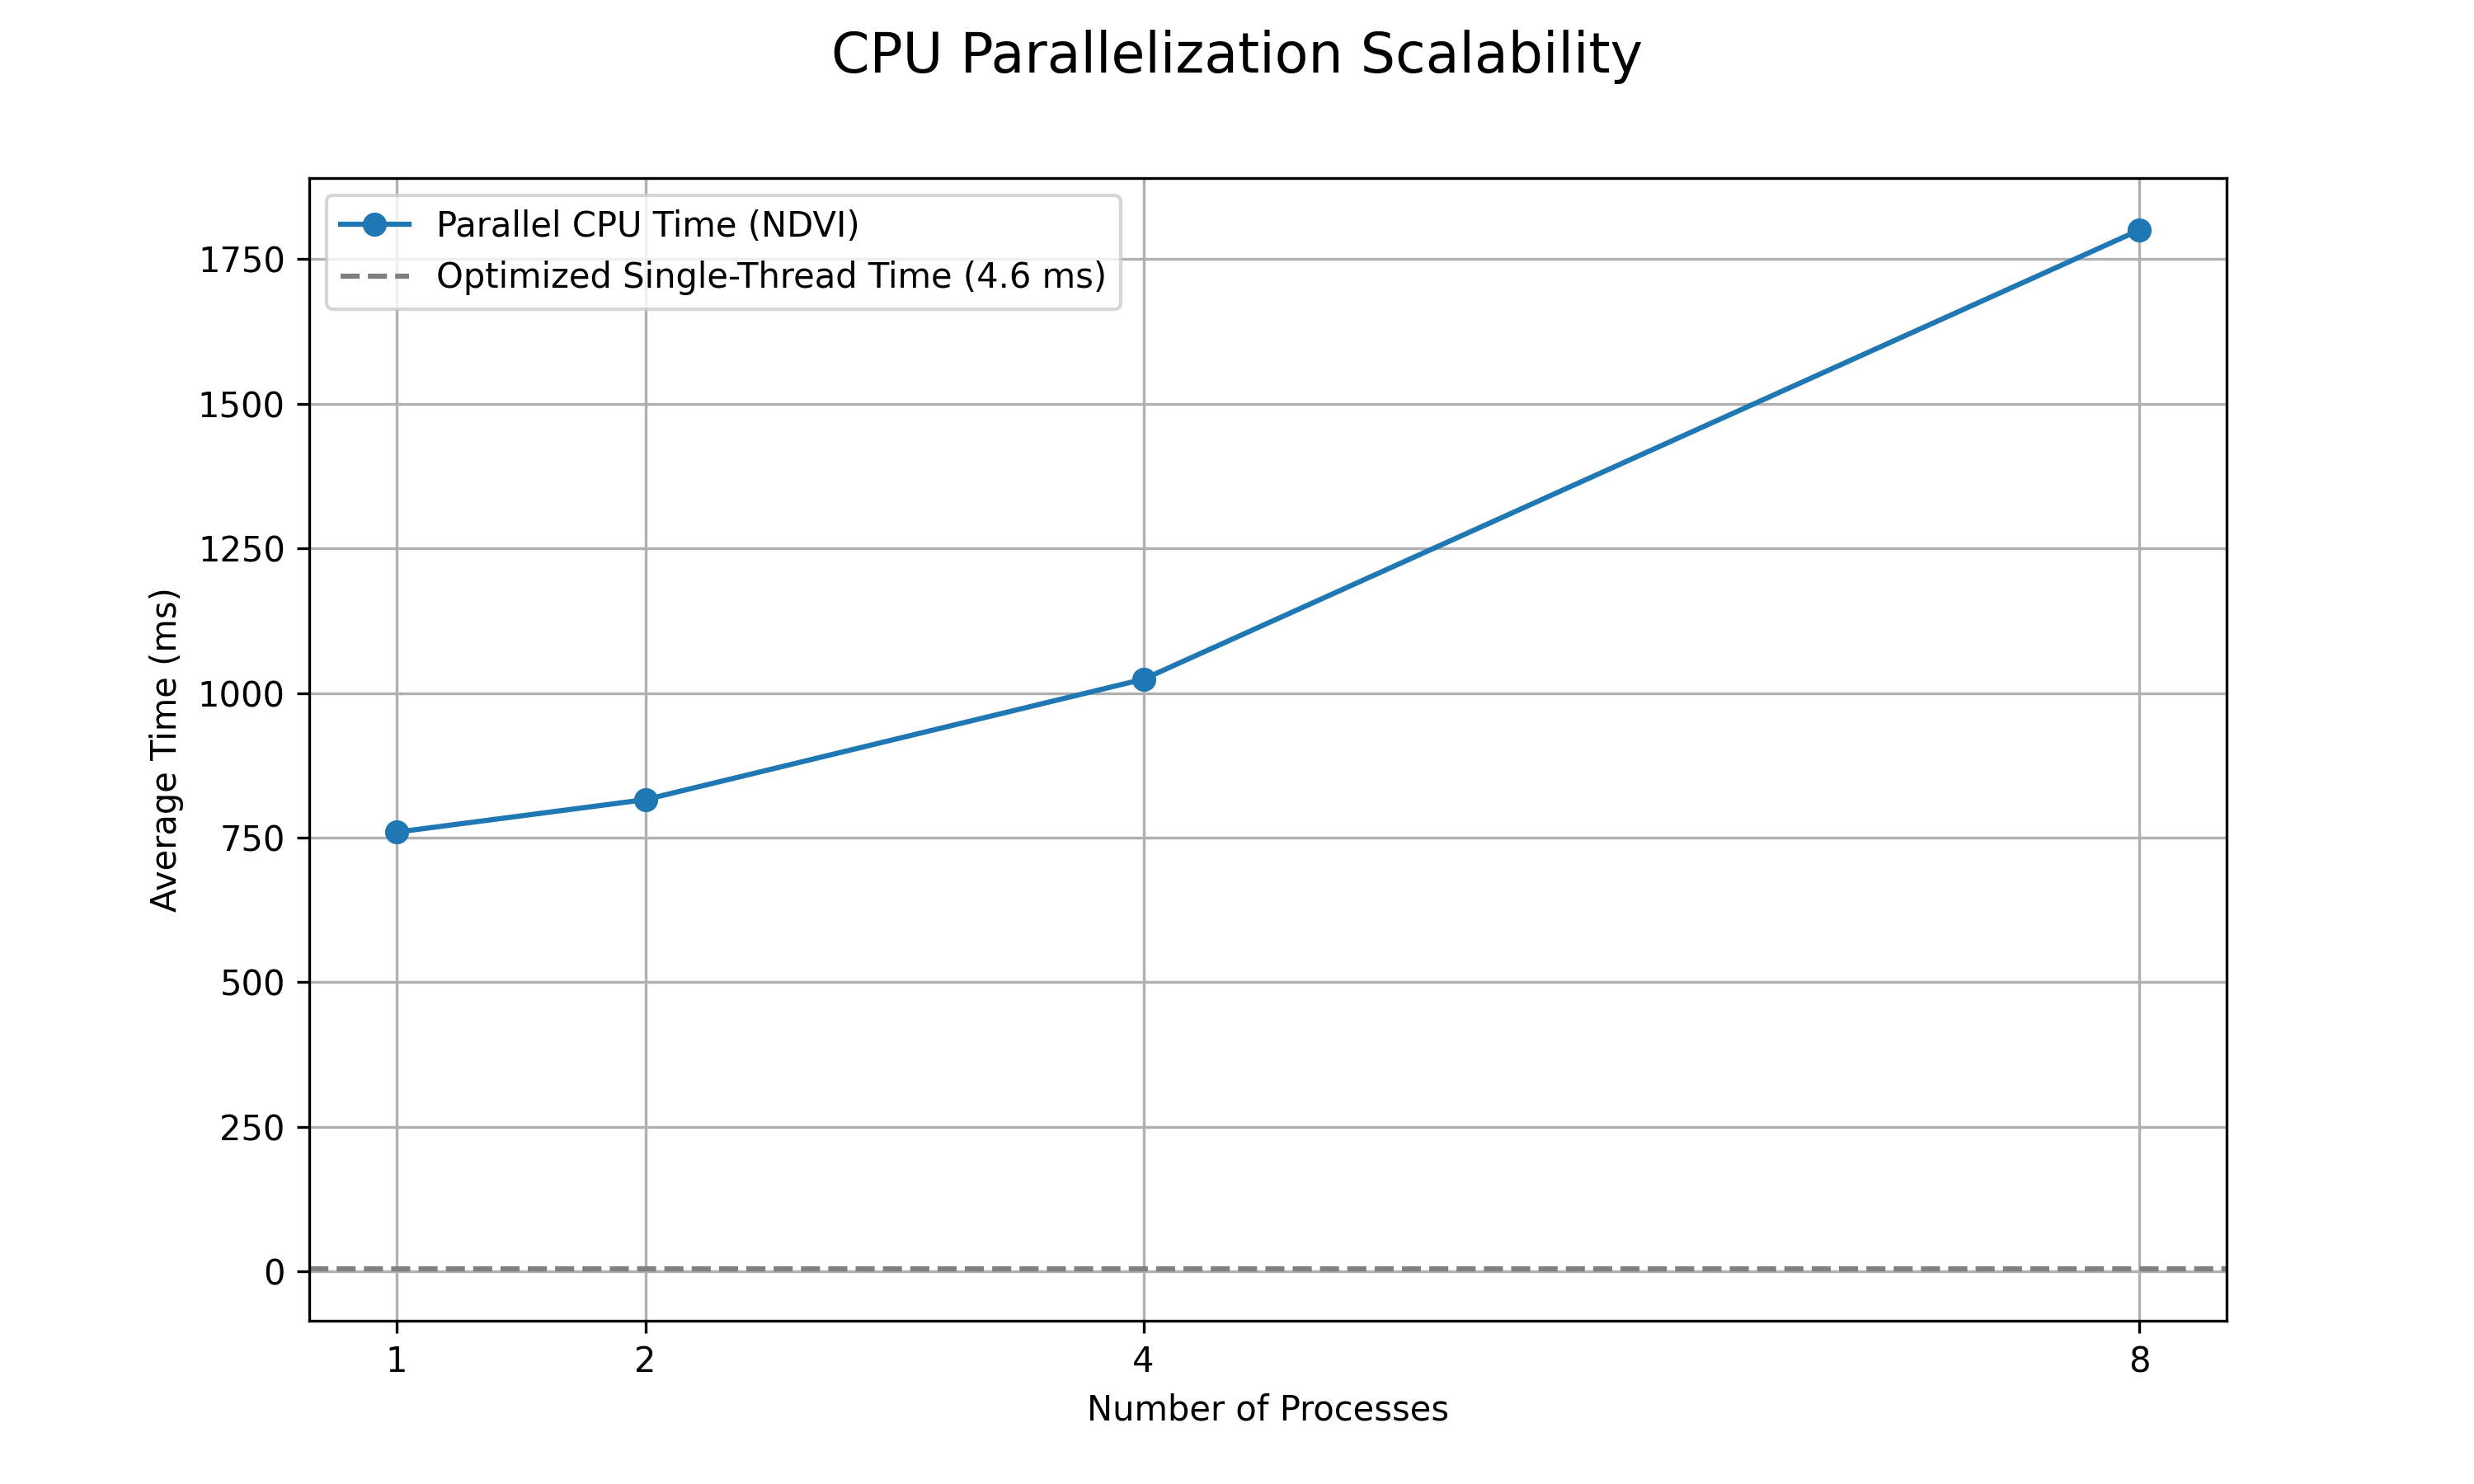
\includegraphics[width=0.8\textwidth]{charts/02_cpu_scalability.png}
    \caption{Analiza skalowalności implementacji równoległej na CPU.}
    \label{fig:cpu_scaling}
\end{figure}

\begin{figure}[H]
    \centering
    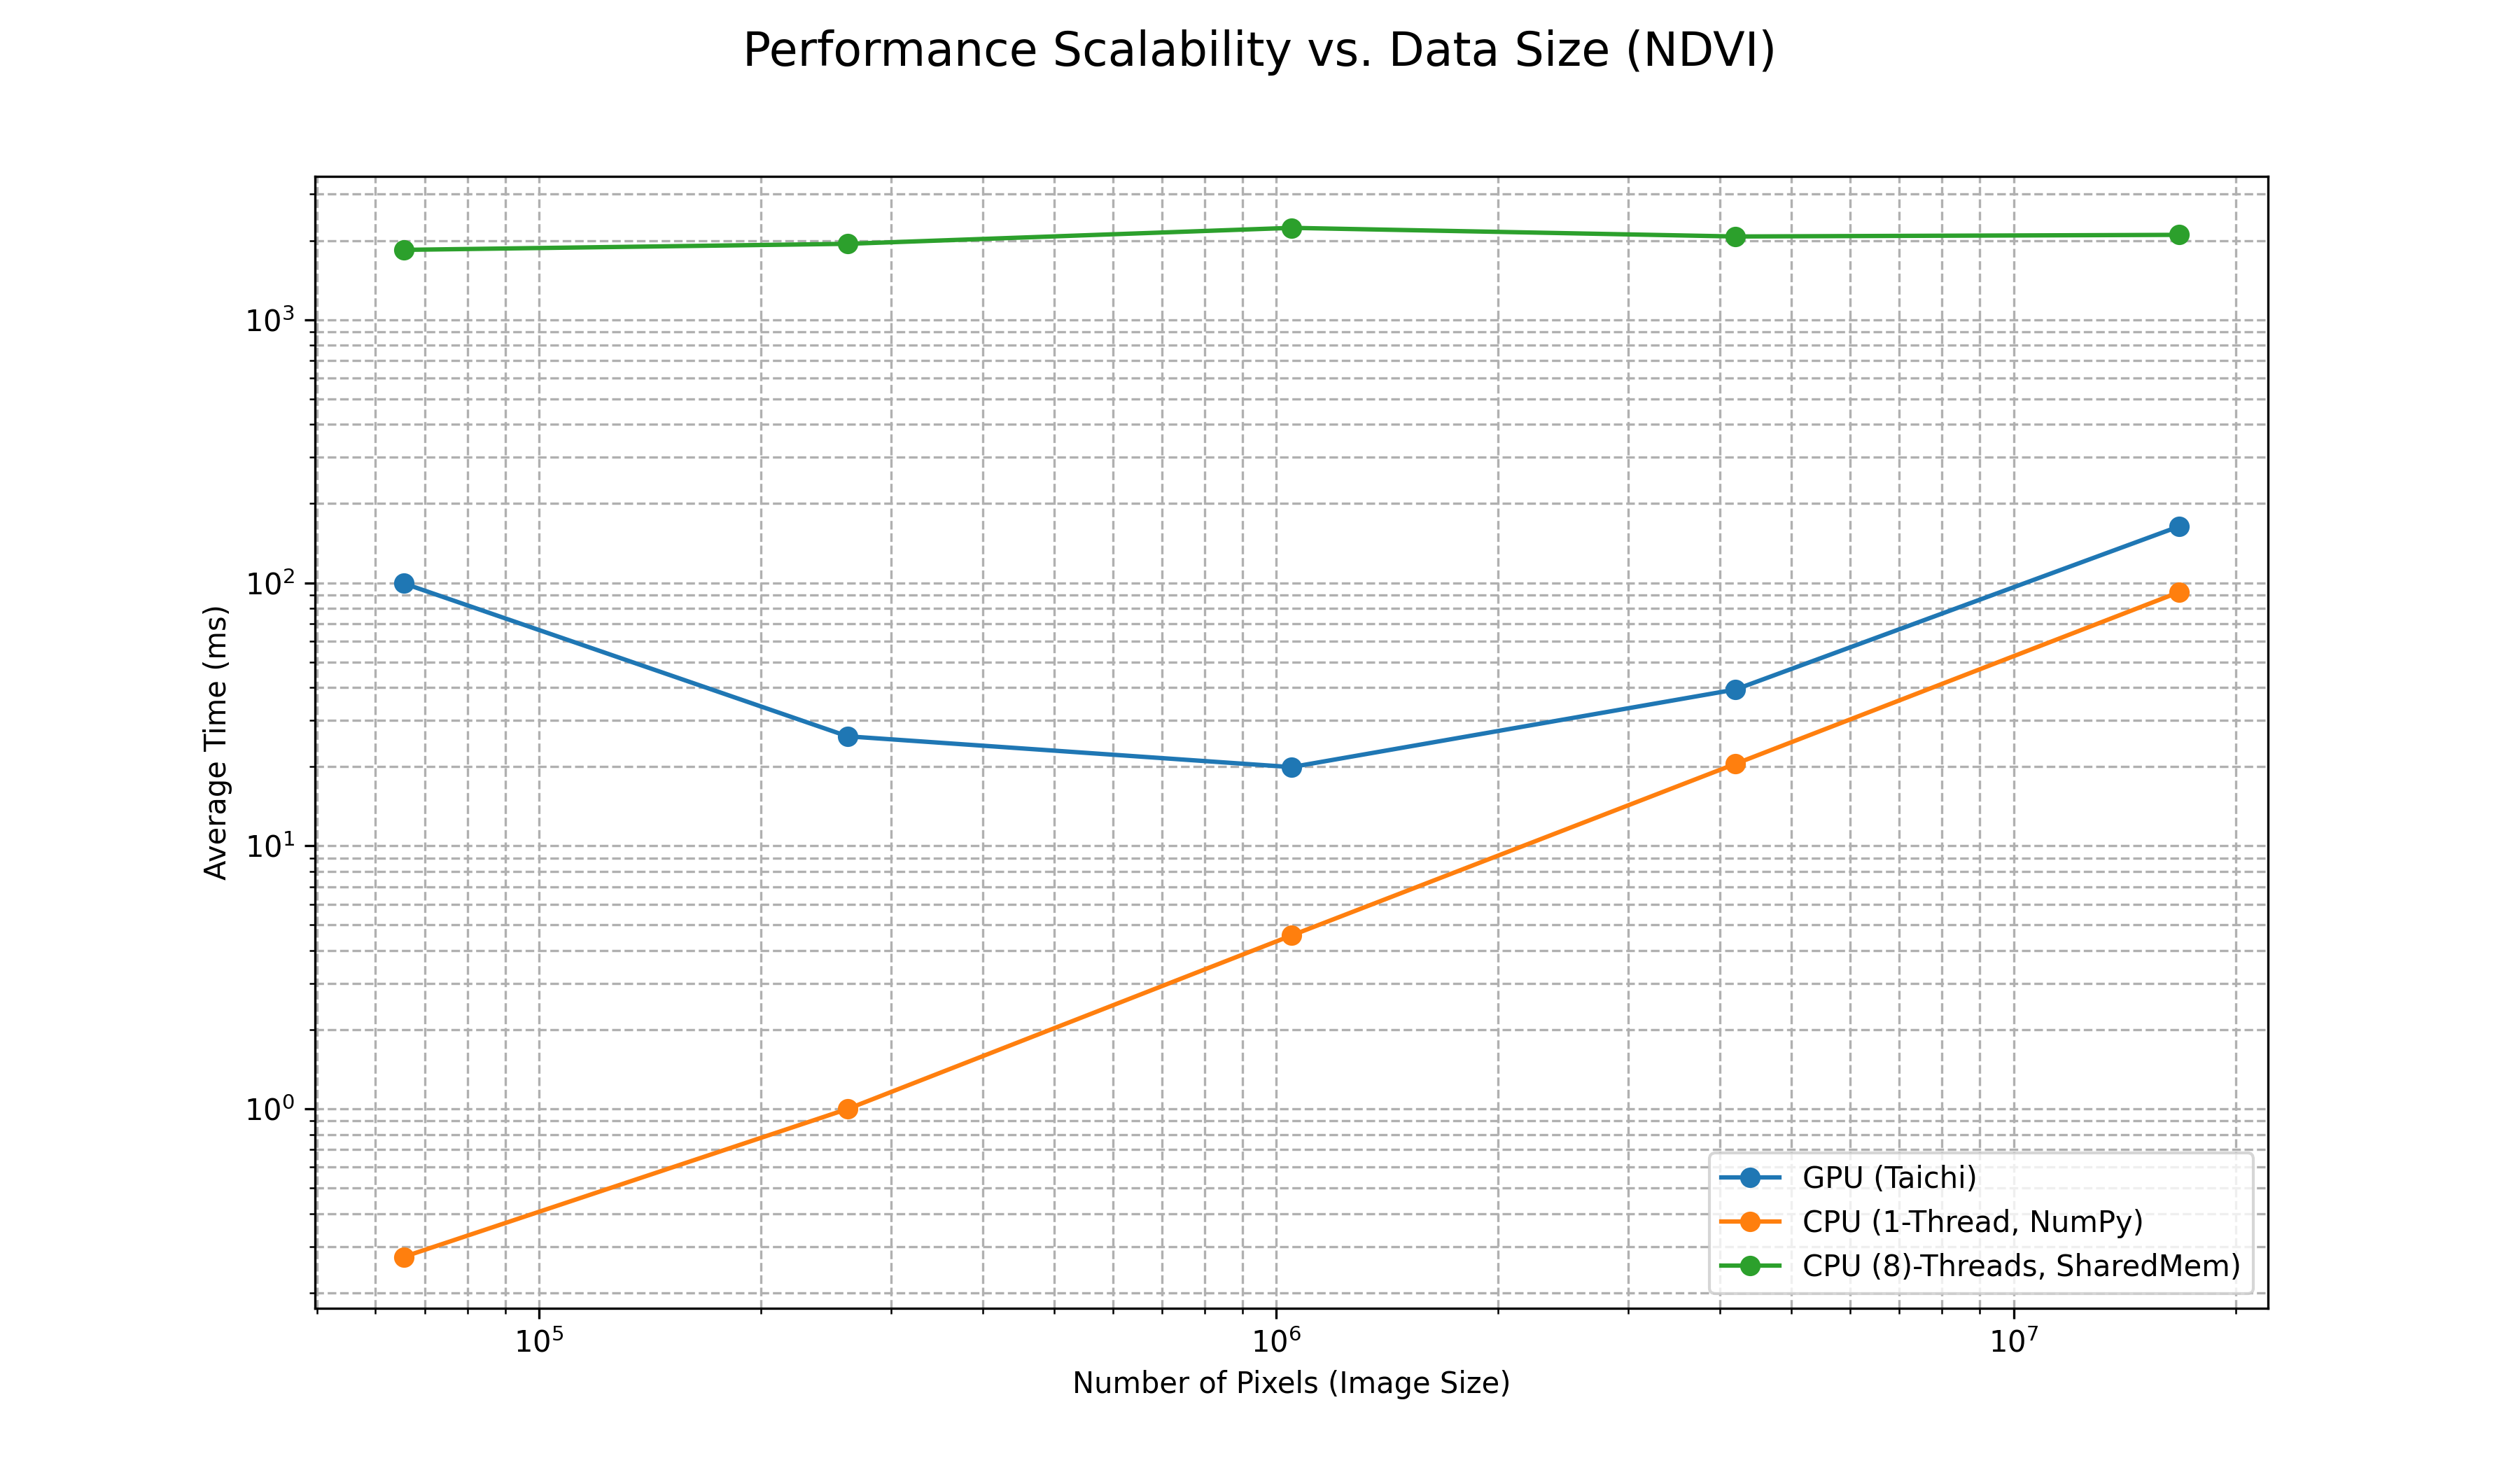
\includegraphics[width=\textwidth]{charts/03_size_scalability_ndvi.png}
    \caption{Skalowalność wydajności w zależności od rozmiaru danych (NDVI).}
    \label{fig:size_scaling_ndvi}
\end{figure}

\begin{figure}[H]
    \centering
    \includegraphics[width=\textwidth]{charts/03_size_scalability_ndmi.png}
    \caption{Skalowalność wydajności w zależności od rozmiaru danych (NDMI).}
    \label{fig:size_scaling_ndmi}
\end{figure}

\begin{figure}[H]
    \centering
    \includegraphics[width=0.8\textwidth]{charts/04_gpu_overhead.png}
    \caption{Analiza narzutu inicjalizacyjnego (warm-up) dla GPU.}
    \label{fig:gpu_overhead}
\end{figure}

\begin{figure}[H]
    \centering
    \includegraphics[width=0.8\textwidth]{charts/05_memory_usage.png}
    \caption{Szczytowe zużycie pamięci RAM przez proces główny.}
    \label{fig:memory}
\end{figure}

\newpage

\section{Interpretacja i wnioski}
Przeprowadzone testy dostarczyły szeregu wnikliwych obserwacji, które pozwalają na sformułowanie kluczowych wniosków dotyczących wydajności i zasadności stosowania różnych technik przetwarzania równoległego dla analizowanego problemu.

\subsection{Wniosek 1: Zoptymalizowany CPU jest najszybszy dla małych i średnich zadań}
Jak widać na Rysunku \ref{fig:overview}, dla standardowego zadania (obraz 1024x1024), wysoce zoptymalizowana, jednowątkowa implementacja oparta na NumPy jest bezkonkurencyjnie najszybsza. Dzieje się tak, ponieważ obliczenia są na tyle proste, że koszt narzutu (overhead) związany z transferem danych do GPU lub zarządzaniem pulą procesów na CPU jest znacznie większy niż zysk z samego zrównoleglenia.

\subsection{Wniosek 2: Przetwarzanie równoległe na CPU ponosi znaczący koszt narzutu}
Rysunek \ref{fig:cpu_scaling} doskonale ilustruje problem narzutu w~`multiprocessing`. Czas wykonania dla jednego procesu w puli jest drastycznie wyższy niż dla wersji jednowątkowej bez puli. Ten ogromny koszt wynika z konieczności tworzenia nowych procesów, konfiguracji pamięci dzielonej i komunikacji międzyprocesowej. Mimo że implementacja poprawnie skaluje się wraz z dodawaniem kolejnych procesów (czas maleje), nigdy nie jest w stanie zniwelować początkowego narzutu i pokonać wydajności czystego NumPy dla tego zadania.

\subsection{Wniosek 3: GPU staje się opłacalne dopiero przy odpowiednio dużym rozmiarze problemu}
Analiza skalowalności w zależności od rozmiaru danych (Rysunki \ref{fig:size_scaling_ndvi} i \ref{fig:size_scaling_ndmi}) jest najważniejszym wynikiem projektu. Obserwujemy, że linia wydajności GPU (niebieska) ma mniejsze nachylenie niż linia CPU (pomarańczowa), co oznacza, że lepiej radzi sobie z rosnącym obciążeniem. Widzimy wyraźny \textbf{punkt przełamania (break-even point)} w okolicach \(2 \cdot 10^6\) pikseli. Poniżej tego progu, zoptymalizowany CPU jest szybszy. Powyżej tego progu, zysk z masowego zrównoleglenia na GPU zaczyna przewyższać stały koszt transferu danych, czyniąc GPU metodą wydajniejszą dla bardzo dużych zbiorów danych.

\subsection{Wniosek 4: Analiza narzutu GPU i zużycia pamięci}
Rysunek \ref{fig:gpu_overhead} potwierdza istnienie kosztu "rozgrzewki" GPU. Pierwsze uruchomienie jest znacznie wolniejsze z powodu kompilacji JIT. Rysunek \ref{fig:memory} pokazuje z kolei kompromisy w zarządzaniu pamięcią. Metoda GPU odciąża systemową pamięć RAM, przenosząc dane do VRAM, co może być zaletą w systemach z ograniczonymi zasobami.

\subsection{Wniosek ogólny: Wybór metody zależy od kontekstu}
Nie istnieje jedna, uniwersalnie najlepsza metoda. Wybór optymalnej strategii zależy od konkretnego przypadku użycia:
\begin{itemize}
    \item \textbf{Interaktywna analiza małych obszarów:} Zdecydowanie najlepszym wyborem jest zoptymalizowany, jednowątkowy CPU (NumPy) ze względu na minimalny czas latencji.
    \item \textbf{Przetwarzanie wsadowe bardzo dużych obrazów:} Dla zadań przekraczających "punkt przełamania", GPU oferuje najwyższą przepustowość i jest metodą preferowaną.
    \item \textbf{Efektywność energetyczna:} Dla zadań, gdzie CPU jest szybsze, jest ono również znacznie bardziej efektywne energetycznie.
\end{itemize}
Nasze wyniki podkreślają, jak kluczowe jest zrozumienie charakterystyki problemu (złożoność obliczeniowa vs. obciążenie I/O) oraz narzutów platformy przy projektowaniu systemów o wysokiej wydajności.

\section{Jak uruchomić program}
Aby uruchomić aplikację, należy postępować zgodnie z poniższymi krokami:

\begin{enumerate}
    \item Sklonować repozytorium projektu i przejść do jego głównego katalogu.
    \item Zainstalować wszystkie wymagane biblioteki za pomocą menedżera pakietów pip:
    \begin{lstlisting}[language=bash]
pip install -r requirements.txt
    \end{lstlisting}
    
    \item Stworzyć plik \texttt{.env} w głównym katalogu projektu. Plik ten będzie zawierał \textbf{jedynie} sól kryptograficzną, która jest niezbędna do odszyfrowania danych logowania. Dla celów testowych i odtworzenia wyników, należy użyć poniższej wartości:
    \begin{lstlisting}
SENTINEL_SALT="385d0b98fb81618a8d5165a2c25300e26217c22661ca9ada7cde877075184219"
    \end{lstlisting}
    
    \item Przygotować własne dane uwierzytelniające (Client ID oraz Client Secret) do API Sentinel Hub. Instrukcje, jak je uzyskać, znajdują się w oficjalnej dokumentacji: \url{https://docs.sentinel-hub.com/api/latest/api/overview/authentication/}.
    
    \item Przy pierwszym uruchomieniu, aplikacja poprosi o podanie uzyskanych danych oraz o hasło, które posłuży do ich zaszyfrowania i bezpiecznego przechowania w pliku \texttt{sentinel\_config.enc}. Dla celów ewaluacji projektu, w repozytorium znajduje się już gotowy plik \texttt{sentinel\_config.enc}, do którego hasło zostanie udostępnione osobno.
    
    \item Uruchomić główną aplikację za pomocą polecenia z \textbf{głównego katalogu projektu}:
    \begin{lstlisting}[language=bash]
python -m src.main
    \end{lstlisting}
    \textit{Uwaga: Użycie flagi \texttt{-m} jest kluczowe, ponieważ zapewnia, że Python poprawnie rozpoznaje strukturę pakietów w folderze \texttt{src}.}
\end{enumerate}

\subsection{Uruchamianie skryptów testowych (opcjonalne)}
Aby przeprowadzić testy wydajności i pamięci, należy najpierw wygenerować dane testowe, a następnie uruchomić skrypt profilujący. Oba skrypty należy uruchamiać z \textbf{głównego katalogu projektu}.

\begin{enumerate}[label*=\arabic*.]
    \item Generowanie danych testowych o różnej skali:
    \begin{lstlisting}[language=bash]
python -m src.scripts.generate_scaled_data
    \end{lstlisting}
    \item Uruchomienie testów zużycia pamięci (wymaga \texttt{memory-profiler}):
    \begin{lstlisting}[language=bash]
python -m memory_profiler src.scripts.run_memory_tests
    \end{lstlisting}
\end{enumerate}


\printbibliography[heading=bibintoc]

\end{document}